\documentclass{article}

\usepackage[utf8]{inputenc}
\usepackage{blindtext}
\usepackage{graphicx}
\usepackage{float} % Elimina la condicion de flotante de las imagenes
\usepackage[english, activeacute]{babel}
\usepackage{amsmath}
\usepackage{etoolbox,fancyhdr,xcolor} % Colores
\usepackage[hidelinks]{hyperref} % Indice dinámico
\usepackage[a4paper]{geometry}
\usepackage{listings} % Para mostrar fragmentos de código.
\usepackage{multicol}

\title{Assignment 1}
\author{José Manuel Izquierdo Ramírez}

\newcommand{\headrulecolor}[1]{\patchcmd{\headrule}{\hrule}{\color{#1}\hrule}{}{}}
\newcommand{\footrulecolor}[1]{\patchcmd{\footrule}{\hrule}{\color{#1}\hrule}{}{}}
\pagestyle{fancy}
\fancyhf{}% Clear header/footer
\fancyhead[L]{\textsl{\leftmark}}
\fancyfoot[C]{\thepage}% \fancyfoot[R]{\thepage}
\renewcommand{\headrulewidth}{0.4pt}% Default \headrulewidth is 0.4pt
\renewcommand{\footrulewidth}{0.4pt}% Default \footrulewidth is 0pt
\headrulecolor{cyan!70}% Set header rule colour to 70% red.
\footrulecolor{cyan!70}
\renewcommand{\sectionmark}[1]{\markboth{#1}{}}
\renewcommand{\subsectionmark}[1]{\markright{#1}}

% Multicol
\setlength{\columnseprule}{0.4pt}
\def\columnseprulecolor{\color{cyan!70}}

\begin{document}

    \begin{titlepage}
        
        \centering
        {\LARGE\bfseries Assignment 1\par}
        \vspace{0,5cm}
        {\itshape\Large Metaheuristics \par}
        \vspace{0,5cm}        

        %{\large \today\par}

    \end{titlepage}
    
    \begin{index}
        \tableofcontents
        \listoffigures
    \end{index}

    \newpage
    
    \section{Exercise 1.}
    \subsection{How does this algorithm behave as we increase the complexity of the problem (number of cities in the TSP)?}

        For this question I have evaluated the algorithm measuring the time and the legnth of the final path, to do this I 
        have done the mean of five iterations for each city using eleven cities between 5 and 150.

        \begin{figure}[H]

            \centering
            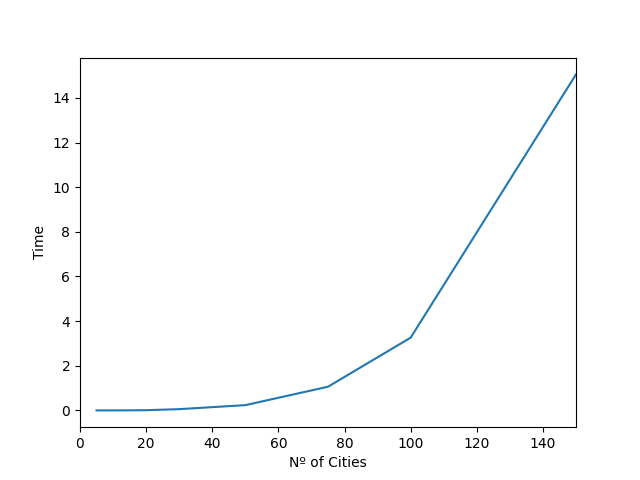
\includegraphics[width=0.5\textwidth]{../media/01.TSP-cities-time.png}
            \caption{Time complexity of Hill Climbing}
            \label{Time complexity of Hill Climbing}

        \end{figure}

        From this figure we can say that the complexity of the algorithm increases exponentially as the number of cities increases.

        \begin{figure}[H]

            \centering
            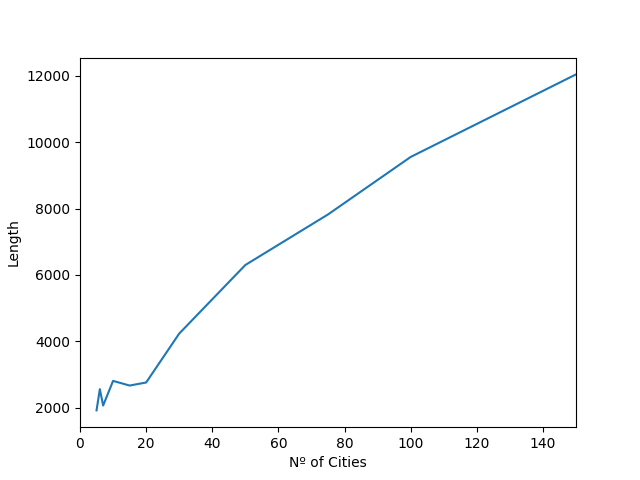
\includegraphics[width=0.5\textwidth]{../media/02.TSP-cities-length.png}
            \caption{Length of final patbh TSP problem}
            \label{Length of final patbh TSP problem}

        \end{figure}

        From this figure we can say that obviously the more cities there are the longer the path will be, however it seems that the heuristic 
        are finfing good solutions because the slope does not increase too much.


    \subsection{Do you always get the best solution? Why? What does it depend on?}

        We do not obtain always the best solution, cause of the first randomly generated solution.
        Sometimes the algorithm get trapped on a local maximum and it never reachs the global maximum.


    \subsection{Modify the code to start the search again from another initial solution (Iterated local search). Have you managed to improve? Why?}
        
        It obteins better results but needs more computation time.
        On my case I do it for 1,10 and 100 iterations.

        Doing that It does not matter if the first random solution is not good, because along the execution of the algorithm it can reach a better neighbour.
        For each iteration it compares if the solution given is better than the best solution ever and if it is better it store the value of it.

        \begin{figure}[H]

            \centering
            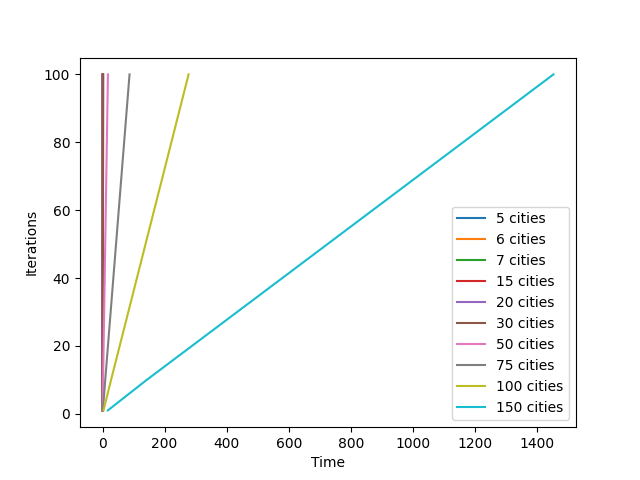
\includegraphics[width=0.5\textwidth]{../media/03.TSP-iterative.png}
            \caption{Computation time changing the iterations}
            \label{Computation time changing the iterations}

        \end{figure}

    \newpage

    \section{Exercise 2.}

        \subsection{How does this algorithm behave as we increase the problem (number of cities in
    the TSP)?}
    
        \subsection{Do you always get the best solution? Why? What does it depend on?}
    
        \subsection{Analyze how the behavior of the algorithm varies as we change the stop criteria
    and the initial temperature.}
    
        \subsection{Modify the code to use different cooling functions}
    
            \subsubsection{Logarithmic.}
    
            \subsubsection{Geometric.}
    
        \subsection{How do these functions affect the final results? Why? Help yourself by representing the values of these functions. Look for new features and compare them to the old ones.}
    
        \subsection{How would you improve the algorithm? For example, reheating so often. Modify
    the code with this and any other improvement you guess is appropriate. Analyze
    the results.}

 
\end{document}